\documentclass[letterpaper]{article}

\usepackage{natbib,alifeconf}  %% The order is important
\usepackage{amsmath}
\usepackage{bbm}
\newcommand{\norm}[1]{\left\Vert #1\right\Vert}
\usepackage{url}

\usepackage{subcaption}
\graphicspath{{images/}}
% *****************
%  Requirements:
% *****************
%
% - All pages sized consistently at 8.5 x 11 inches (US letter size).
% - PDF length <= 8 pages for full papers, <=2 pages for extended
%    abstracts.
% - Abstract length <= 250 words.
% - No visible crop marks.
% - Images at no greater than 300 dpi, scaled at 100%.
% - Embedded open type fonts only.
% - All layers flattened.
% - No attachments.
% - All desired links active in the files.

% Note that the PDF file must not exceed 5 MB if it is to be indexed
% by Google Scholar. Additional information about Google Scholar
% can be found here:
% http://www.google.com/intl/en/scholar/inclusion.html.


% If your system does not generate letter format documents by default,
% you can use the following workflow:
% latex example
% bibtex example
% latex example ; latex example
% dvips -o example.ps -t letterSize example.dvi
% ps2pdf example.ps example.pdf


% For pdflatex users:
% The alifeconf style file loads the "graphicx" package, and
% this may lead some users of pdflatex to experience problems.
% These can be fixed by editing the alifeconf.sty file to specify:
% \usepackage[pdftex]{graphicx}
%   instead of
% \usepackage{graphicx}.
% The PDF output generated by pdflatex should match the required
% specifications and obviously the dvips and ps2pdf steps become
% unnecessary.


% Note:  Some laser printers have a serious problem printing TeX
% output. The use of ps type I fonts should avoid this problem.


\title{Generating urban morphologies at large scales}
\author{Juste Raimbault$^{1,2,3,*}$ \and Julien Perret$^{1,4}$ \\
\mbox{}\\
$^1$UPS CNRS 3611 ISC-PIF\\
$^2$CASA, UCL\\
$^3$UMR CNRS 8504 G{\'e}ographie-cit{\'e}s\\
$^4$Univ. Paris-Est, LaSTIG STRUDEL, IGN, ENSG\\\medskip
* juste.raimbault@polytechnique.edu} % email of corresponding author

% For several authors from the same institution use the same number to
% refer to one address.
%
% If the names do not fit well on one line use
%         Author 1, Author 2 ... \\ {\Large\bf Author n} ...\\ ...
%
% If the title and author information do not fit in the area
% allocated, place \setlength\titlebox{<new height>} after the
% \documentclass line where <new height> is 2.25in



\begin{document}
\maketitle

\begin{abstract}
% Abstract length should not exceed 250 words
  At large scales, typologies of urban form and corresponding generating processes remain an open question with important implications regarding urban planning policies and sustainability.
  We propose in this paper to generate urban configurations at large scales, typically of districts, with morphogenesis models, and compare these to real configurations according to morphological indicators.
  Real values are computed on a large sample of districts taken in European urban areas.
  We calibrate each model and show their complementarity to approach the variety of real urban configurations, paving the way to multi-model approaches of urban morphogenesis.
\end{abstract}


%%%%%%%%%%%%%%%%%%%%%
\section{Introduction}


The study of forms of the built environment, and more precisely of the urban environment, has been the subject of different disciplines such as architecture, urban planning, or geography, with different approaches corresponding to various scales and processes \citep{moudon1997urban,gauthier2006mapping,kropf2009aspects}.
Establishing typologies of urban morphologies, and understanding their link with underlying urban growth processes, is nowadays a crucial issue for sustainability as a large majority of the world population live in cities and energy consumption is closely related to urban form \citep{newman2000sustainable}.%Automobile dependence


Although there is neither a unified definition of urban form, nor unified generative models and quantitative indicators to measure it, several approaches are close to the spirit of artificial life and generative social science.
Procedural modeling \citep{watson2008procedural} aims at generating realistic cities, but is mostly focused on the visual impression given and does not consider realistic generative processes.
It is furthermore developed largely at larger scales than the one of the district \citep{Parish:2001:PMC:383259.383292}.
Approaches linked to urban planning have focused on the spatial distribution of land-use, at multiple scales \citep{liu2017future}, and proposed cellular automata models for urban sprawl, generally at the scale of the metropolitan area \citep{herold2003spatiotemporal}.

%Merrell, P., Schkufza, E., & Koltun, V. (2010, December). Computer-generated residential building layouts. In ACM Transactions on Graphics (TOG) (Vol. 29, No. 6, p. 181). ACM. -> intra building (mimic architecture)

% Horner, M. W. (2007). A multi-scale analysis of urban form and commuting change in a small metropolitan area (1990–2000). The Annals of Regional Science, 41(2), 315-332. : not really multi-scale ? + based on land-use


This paper proposes a first step towards a systematic understanding of generative models of the urban form, at a large scale.
The approach taken here is similar to the one taken by \cite{raimbault2018calibration}, which computes urban form indicators at a mesoscopic scale (metropolitan area) and calibrates a reaction-diffusion morphogenesis model.
We consider real urban configurations at the scale of the district (fixed spatial window of 500m), compute their morphological characteristics, and use these measures to calibrate different generative models of urban layouts at the same scale.
Our contribution is twofold: (i) we synthesize a set of indicators relevant at this scale, and compute them on a large sample of real urban configurations in European urban areas; (ii) we provide three different generative models
% on drop le random ?

The rest of this article is structured as follows.
First, we present the methods used in our work, including the measures allowing the comparison of urban forms, the proposed generative models and the method used to retrieve real urban configurations.
The results of the proposed approach are then explained together with the tools used in the calibration of the models.
Finally, the results are discussed.

%%%%%%%%%%%%%%%%%%%%%
\section{Methods} \label{sec:methods}

\subsection{Quantifying urban forms}

% literature on typologies ? not the main purpose of the paper
\cite{2017arXiv170902939M} deep learning classification of roads

% Webster, C. J. (1995). Urban morphological fingerprints. Environment and Planning B: Planning and design, 22(3), 279-297.
\citep{webster1995urban}

% + fractal dims etc

\cite{boeing2018measuring} %measures
\cite{fumega2014identification} %typology, metrics for Urban Energy And Climate Change Analysis
\cite{rode2014cities} %urban morphology and residential heat-energy demand

In practice, we use a variety of indicators capturing different aspects, each being detailed below.

\subsubsection{Basic indicators}
% building area, density, moran, average distance, number of buildings (components), average building area


\subsubsection{Network indicator}
% avg detour, average component area


\subsubsection{Mathematical morphology indicators}
% dilation steps, erosion steps
% closing / opening not included - would require profile = f(kernel size)










\subsection{Real urban morphologies}

% osm buildings



\subsection{Generative models}

We consider the local urban space as a square grid with cells $1 \leq i \leq N$, and an urban configuration is a binary function $s_i \in \{0;1\}$ on these cells.
% TODO justify the raster configuration (wouldnt be more logical to have vector generators at this scale ? discuss on "patches" : we do not care about even smaller details in buildings (as architects could do), but on the spatial distribution of free/occupied space at the granularity of patches. consistent with morpho indicators as they are computed, specifically for morpho math.


%%%%%%%%%%%%%%
\begin{figure}
    \centering
    \begin{subfigure}[b]{0.2\textwidth}
        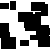
\includegraphics[width=\textwidth]{blocks}
        \caption{Blocks}
        \label{fig:blocks}
    \end{subfigure}
    \begin{subfigure}[b]{0.2\textwidth}
        
\includegraphics[width=\textwidth]{expMixture}
        \caption{Kernel mixture}
        \label{fig:mixture}
    \end{subfigure}
    \begin{subfigure}[b]{0.2\textwidth}
        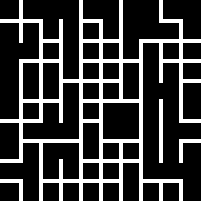
\includegraphics[width=\textwidth]{percolation}
        \caption{Network percolation}
        \label{fig:percolation}
    \end{subfigure}
    \begin{subfigure}[b]{0.2\textwidth}
        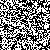
\includegraphics[width=\textwidth]{random}
        \caption{Random}
        \label{fig:random}
    \end{subfigure}
    \caption{Patterns produced by the synthetic generators.}
    \label{fig:generators}
\end{figure}
%%%%%%%%%%%%%%



\subsubsection{Blocks generator}

The most simple ``realistic'' generator is similar to procedural modeling and distributes building blocks into the space. Given a number $N_B$ of blocks, random positions are drawn and block of a random height and width (with minimal value $m_B$ and maximal value $M_B$ as parameters) are placed at these.


\subsubsection{Kernel mixture generator}

Kernel mixture are a classical way to represent the spatial distribution of population density in an urban area \citep{anas1998urban}. They remain relevant at our scale, as they can be interpreted as a superposition of ``density hotspots'', as can the planning or the self-organization of a district can be. Given a number of centers $N_K$, $\vec{x}_{1\leq j \leq N_K}$ random position are drawn in the grid, at which kernels are applied, such that $s_i = \mathbbm{1}_{d_i \geq \theta_K}$ where the density $d_i$ for the point at position $\vec{x}_i$ is given by
\begin{equation}
    d_i = \frac{1}{N_K}\cdot \sum_j \exp{\left(-\norm{\vec{x}_j - \vec{x}_i}/d_K\right)} 
\end{equation}
where $d_K$ is a range parameter giving the extent of kernels.

\subsubsection{Network percolation model}

The last generator we used is based on network percolation, in the spirit of capturing the constraints imposed by flows traversing a given urban area. While the two previous generator were based on building processes, this one relies on streets, and thus on processes linked to transportation. The idea is to link a fixed number $N_P$ of border points, which can be understood as entrances/exits of the area. Starting with a grid network 


% note that our generators will be "fairly compared" in terms of calibration, as they have the same number of parameters



%%%%%%%%%%%%%%%%%%%%%
\section{Results} \label{sec:results}

Simulation results and real measures are available on the dataverse repository at \url{https://doi.org/10.7910/DVN/LGK0US}. Source code is available on the git repository of the project at \url{https://github.com/openmole/spatialdata}.


%%%%%%%%%%%
\subsection{Real measures}

We compute the morphological indicators given above on a large sample on real urban areas. For practical computational reasons, we restrain our geographical area of study to European urban areas as provided by \cite{}. We expect to already have a good representativity, although not universal, of existing urban forms with this sample, as it is known that European cities already have a significant morphological diversity \citep{le2015forme}. We collect building layouts from OpenStreetMap, as this source has been shown to have a good quality especially in Europe \citep{mooney2010towards}. Using the \texttt{osmosis} tool, buildings are filtered from the openstreetmap raw dump for Europe (downloaded from \url{http://download.geofabrik.de/} in March 2019) and inserted into a Postgis database, which can then be efficiently queried for a specific bounding box.
%Our tool also provide a direct access to the classic and overpass API % not necessary ?
We sample $N=xx$ points into polygons corresponding to urban areas, first by selecting the area with a uniform selection weighted by population of areas, then by drawing uniform spatial coordinates within the polygon with a polygon sampling heuristic. % TODO clarify the polygon sampler


%  dim(real)
% 17612    16

%                           PC1    PC2     PC3
% Cumulative Proportion  0.7031 0.8592 0.92755


We show in Fig.~\ref{fig:realtypology} a typology of urban areas obtained from these measures.
% TODO typology of urban areas ?

%%%%%%%%%%%%%%
\begin{figure}
    \centering
%    \includegraphics{}
    \caption{Typology of morphological profiles of European urban areas.}
    \label{fig:realtypology}
\end{figure}
%%%%%%%%%%%%%%




%%%%%%%%%%%
\subsection{Direct sampling}

A first simulation experiment provides an insight into the patterns produced by the different generators in the morphological space. We sample the parameter space using a Latin Hypercube Sampling, with 10000 points for each generator respectively, and with 100 stochastic repetitions for each parameter point. The corresponding point cloud is shown in a reduced dimension in Fig.~\ref{fig:lhs}.

%%%%%%%%%%%%%%
\begin{figure}
    \centering
%    \includegraphics{}
    \caption{Comparison of real morphologies with patterns produced by the synthetic generators.}
    \label{fig:lhs}
\end{figure}
%%%%%%%%%%%%%%


%%%%%%%%%%%
\subsection{Calibration with Genetic algorithms}

The mapping between generator parameters and the morphological space being highly non-linear, we are not ensured that the proximities observed above fully correspond to the potentialities of generators to generate real forms. Therefore, we proceed here to a calibration of these models.



%%%%%%%%%%%%%%%%%%%%%
\section{Discussion} \label{sec:discussion}

% Towards multi-scale approaches


%%%%%%%%%%%%%%%%%%%%%
%\section{Conclusion}



%%%%%%%%%%%%%%%%%%%%%
\section{Acknowledgements}

Results obtained in this paper were computed on the vo.complex-system.eu virtual organization of the European Grid Infrastructure ( http://www.egi.eu ). We thank the European Grid Infrastructure and its supporting National Grid Initiatives (France-Grilles in particular) for providing the technical support and infrastructure.

\footnotesize
\bibliographystyle{apalike}
\bibliography{biblio} % replace by the name of your .bib file


\end{document}



%%%%%%%
%% Templates

%\begin{figure}[t] % [!tbp] % [ht]
%\begin{center}
%\includegraphics[width=2.2in, angle=90]{fig5.eps}
%\vskip 0.25cm
%\caption{Fitted exponent of power law for 34 runs at mutation rates  between $R=0.0005$ and $R=0.01$ copy errors per instruction  copied. The error bars reflect the standard deviation across the  sample of runs taken at each mutation rate. The solid line is to  guide the eye only.}
%\label{fig5}
%\end{center}
%\end{figure}


%\begin{table}[h]
%\center{
%\begin{tabular}{|c|c|c|c|}\hline
%Name & Result & Bonus $b_i$ & Difficulty\\ \hline\hline
%Echo & I/O   & 1 & --\\
%Xor  & $ A\ {\rm xor}\ B$ &   6 & 4 \\
%Equals &$\neg(A\ {\rm xor}\ B)$&6& 4 \\ \hline
%\end{tabular}
%}
%\vskip 0.25cm
%\caption{Logical calculations on random inputs $A$ and $B$ rewarded,bonuses, and difficulty (in minimum number of {\tt nand} instructionsrequired). Bonuses $b_i$ increase the speed of a CPU by a factor
%$\nu_i=1+2^{b_i-3}$.}
%\end{table}


